
\section{Test Driven Development}

Designing code using a test first approach helps direct the design
of the code in a way that makes it more flexible. This section will
cover how to achive this, along with helpful advice on how to handle
certain aspects of the TDD%
\footnote{Test Driven Development%
} process. As such it will also explain the ways unit tests should
be used and what problems that might occur when attempting to write
unit tests. 

\begin{figure}
\begin{centering}
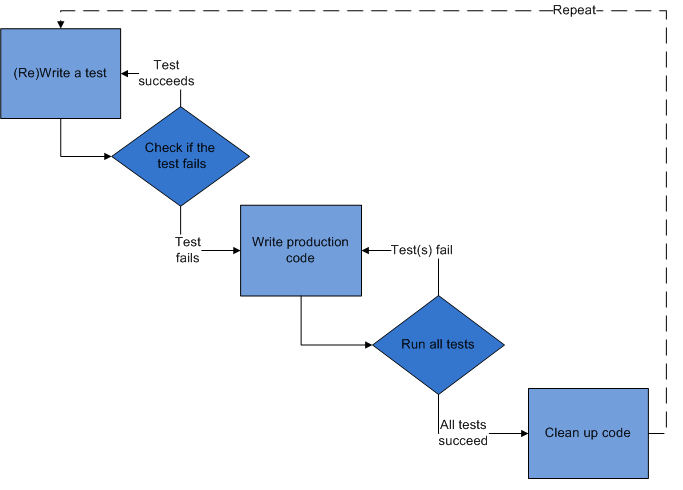
\includegraphics[width=0.7\textwidth]{TestWrittenCycle}
\par\end{centering}

\caption{The cycle of writing tests used to develop production code (from ~\cite{WikiTDD},
\texttt{http://upload.wikimedia.org/wikipedia/en/9/9c/Test-driven\_development.PNG})\label{fig:TestWrittenCycle}}
\end{figure}



\subsection*{The Idea Behind Test Driven Development}

The idea of TDD is to write tests of how the program is supposed to
function before actually writing the program itself. These tests can
be referred to as executable specification, because they specify how
single units of the program are meant to be used.

To get an idea of how a TDD process works, look at fig. \ref{fig:TestWrittenCycle}.
As is shown in the figure, the idea is that you begin the development
of a unit in the program by writing a test. The production code is
then developed with the goal of having the test succeed. Once all
tests succeed, you clean up the code and start the process over, with
developing new features and accompanying tests. After multiple iterations,
you have ensured that not only does your code have all the features
you want, but that those features work as you would expect. Furthermore,
if new features were requested at a later time, it would be quite
easy to simply add new tests and begin development of the new features,
while using the old tests to ensure the old features were not ruined.

By writing the tests first, the developer can easily determine what
the final units should look like. If he did not apply a test first
approach he would have to do a lot more preplanning, as he would have
to state the specifications of the program in some other way. While
a TDD approach will reduce the amount of preplanning required, it
will not completely remove the need for it. It will still be required
to plan such things as the domain model and the components of the
program. 

To give an idea of what the executable specifications obtained through
TDD will look like, we provide the following example:

Assume you were to make a Calculator. Since this is a simple calculator,
it can only do addition, subtraction, multiplication and division.
To specify this calculator, one must create a test for each of its
features:
\begin{itemize}
\item A test showing addition of two numbers 
\item A test showing subtraction of two numbers 
\item A test showing multiplication of two numbers 
\item A test showing division of two numbers
\end{itemize}
This specification will ensure that the final calculator can perform
all these actions or it will not work, thus our tests are enforcing
specified features of the calculator.

However, the great thing about using TDD is that you can go deeper
and specify what the exact outcome should be. Assume that you wanted
to ensure that when the calculator divides by zero, an error is thrown.
To do this, all that is required is to simply add a new test:
\begin{itemize}
\item A test showing that when the calculator divides by zero, an error
is thrown.
\end{itemize}
As is evident, the more tests written for a certain aspect of the
program, the more specified that aspect is. Thus by doing test driven
development, you have essentially done two things at once. First,
you have created a way to test if the features are still functional;
this provides a way to test them if their functionality is changed
at a later date. Second, by making tests you are specifying what the
output of the program should be, thus if others were to try and use
your units in their code, it would be easy for them to understand
the provided functionality by simply inspecting the unit tests you
provide.


\subsection{How to write unit tests}

When following the TDD approach, it is important to properly understand
how to design unit tests, as many problems can arise when writing
them. Most of these problems can be traced to a few common programming
mistakes. A good introduction to using test-driven development is
Misko Hevery's lecture on the subject, see ~\cite{LectureTDD}.

As mentioned in ~\cite{LectureTDD}, there is nothing that can be
said about writing unit tests that would improve the tests, there
is no trick to writing them. However there is a lot that can be said
about designing code, a correctly designed piece of code can make
the process of making a unit test easy, while a badly designed piece
of code can make creating a unit test very difficult, if not impossible.
To understand what these bad design choices are, we will go through
each of them. 


\subsubsection*{Mixing Object creation logic with business logic}

To properly design a test for a given class in the code, you must
be able to instantiate that object. If the object you wish to test
instatiates all its dependencies on construction (in contrast to taking
instantiated dependencies as arguments), you are forced to test all
these dependencies along with the class.

To give an example of this problem, assume you have a \texttt{WebDocument
}class, as shown below:

\begin{alltt}
Class WebDocument 	
    Field: Document 	
    Constructor takes URL 		
        client = new TCPClient() 		
        Document = client.Download(URL)
    Endconstructor 
Endclass
\end{alltt}

In this example the \texttt{WebDocument }creates its own TCP client
which it uses to download a document from an URL. If we were to test
this class we would be forced to setup a TCP connection every single
time. This not only causes the test to be slow it also introduces
uncertainty, as the TCP connection could fail.

This problem can be solved by designing the class so that it requires
the classes to be provided instead of instantiating them itself. This
method is called dependency injection. Consider the following adaptation
of the \texttt{WebDocument} class, which uses dependency injection:

\begin{alltt}
Class WebDocument
    Field: Document 
    Constructor takes Client, URL 		
        Document = Client.Download(URL) 	
    EndConstructor 
EndClass
\end{alltt}

By making this change, the test creator can choose which object is
given as the client. For instance he could use a mock%
\footnote{An object that mimics the behavior of the real object%
} client providing a document of his choosing in the \texttt{Download}
method.

This basically comes down to giving choice to the unit test writer,
without this the unit tester could be required to instantiate almost
the entire program in order to just test a single unit. By using dependency
injection we effectively remove this issue.


\subsubsection*{Global State in the Code}

Whenever you have global state in your units it becomes very difficult
to design tests, as pointed out in ~\cite{LectureSingletons}. This
is because actions done in one test will inadvertently affect the
result of another test. Thus by eliminating all sources of global
state you ensure that the code which you are testing always works
in the same manner.

If the developer is not careful, it is often easy to accidentally
write code with global state in it, since it can the global state
can be quite subtle. By definition, global state occurs every time
a piece of code knows about something that is has no reference to,
thus it has reference to something that is globally accessible.

To illustrate this, consider the following simple test:

\begin{alltt}
Output1 = new A().Calculate() 
Output2 = new B().Calculate() 
Assert(Output1 != Output2)
\end{alltt}

Since a computer is deterministic, the result of asserting that the
two outputs are not equal should always be the same. If the assertion
is sometimes true and sometimes false, then we have a global state.
This means that global state in code is what makes the code non-deterministic.
By its very nature, code that is non-deterministic is untestable,
since a test requires knowing the outcome in advance so it can be
asserted whether the result is the same.

Here we provide two examples of commonly accepted code design that
produces global state:


\subparagraph*{Singletons}

are objects that are only instantiated once. Their instantiation is
located on a global variable, since the variable on which the singleton
is located is global. That means all objects that use the singleton
has their state bound to that of the singleton.


\subparagraph*{Random numbers, Time and date, etc.}

are all cases of objects that hides global state inside them. Thus
if you use them as part of your code without providing a way for a
test to inject them as with other dependencies, you run the risk of
the program being untestable. The problem with these objects are they
usually hide the fact that they use global state, and as such can
easily sneak their way into the code if one is not careful. 


\subsubsection*{Breaking Law of Demeter}

One thing that makes testing difficult is if an object does not ask
for what it needs, but for the objet that can locate what it needs.
The act of asking only what is needed is called Law of Demeter or
principle of least knowledge. The idea is that a unit only needs to
know about its immediate friends; units it doesn\textquoteright{}t
directly work with should be irrelevant to it. Breaking the law of
Demeter is not only considered bad code design, but also makes writing
unit test harder.

When writing code, it is not always immediately obvious when law of
Demeter is violated. In the real world, however, breaking the law
of Demeter often results in absurd situations, and are thus more easily
visible.

As an example (adapted from ~\cite{WikiDemeter}), imagine that you
are in a shop and the cashier asks for 10\texteuro. What would you
do?
\begin{enumerate}
\item Give him a 10\texteuro bill
\item Give him the wallet and let him find the money
\item Give him the location of a hidden treasure which he should locate
and return the difference to you.
\end{enumerate}
As we can see option 2 and 3 clearly violate law of Demeter because
instead of giving what is actually required we give something that
provides what is actually required.

In the example of the \texttt{WebDocument }we ourselves violated law
of Demeter so let us show how we could change the code to remedy this.
The code that breaks law of Demeter:

\begin{alltt}
Class WebDocument 	
    Field: Document 	
    Constructor takes Client, URL 		
        Document = Client.Download(URL) 	
    EndConstructor 
EndClass
\end{alltt}

The modified, more correct code:

\begin{alltt}
Class WebDocument 	
    Field: Document 	
    Constructor takes ADocument 		
        Document = ADocument 	
    EndConstructor 
EndClass
\end{alltt}

As we can see, instead of making \texttt{WebDocument }go locate the
document on some server, we simply make the document a dependency
of the \texttt{WebDocument }class, thus testing of the \texttt{WebDocument
}will not even require a mock server anymore. As such designing the
test just became a lot easier.


\subsection*{Summary}

While a TDD approach will increase the workload of the project as
it will require the developer to write a lot of tests, it adds a lot
of value in return. The most useful feature of TDD is perhaps that
it provides a natural specification of the programs individual units,
which could be hard to properly formulate in words. It also enforces
good code design practices by making it hard to write unit tests for
badly designed code.


\paragraph*{Advantages}
\begin{itemize}
\item Provides test cases for all units, making it easier to see what breaks
when units are introduced or changed
\item Reduces the amount of errors in the final product and as such reduces
time spent debugging
\item Enforces proper code design
\item Provides specification of the code, making it easy for others to understand
\item Makes the writing process of a class easier since you start by stating
what you want from a class, instead of how it works.
\end{itemize}

\paragraph*{Disadvantages}
\begin{itemize}
\item Requires unit testing frameworks to do it properly
\item Has a learning curve for those no familiar with TDD
\item Increases the develop time as all code produced must also have a unit
test to prove it works as expected\end{itemize}

